\documentclass[]{aastex63}

\newcommand{\vdag}{(v)^\dagger}
\newcommand\aastex{AAS\TeX}
\newcommand\latex{La\TeX}
\usepackage{xcolor}
%\received{}
%\revised{}
%\accepted{\today}

%\submitjournal{AJ}

%\shorttitle{}
\shortauthors{Kiker et al.}
%\graphicspath{{./}}

\begin{document}

\title{A Survey of Meteorite-specific Minerals}

\author{Thaddaeus J. Kiker}
\affiliation{Sunny Hills High School, 1801 Lancer Way, Fullerton, CA 92833}

\author{Nina Hooper}
\affiliation{Abrility, 11 York St, Sydney, NSW 2000, Australia}

\author{Martin Elvis}
\affiliation{Harvard-Smithsonian Center for Astrophysics
60 Garden St., Cambridge, 
Massachusetts 02138, USA}

\correspondingauthor{Martin Elvis}
\email{melvis@cfa.harvard.edu}

\submitjournal{RNAAS}

\begin{abstract}
Dozens of exotic materials are found only in meteorites. These “meteorite minerals” are formed in the Solar System’s cold, long-lived, proto-planetary disk, in the slowly cooling cores of planetesimals, and in high-speed collisions. To the best of our knowledge no recent refereed work has aggregated information about minerals only found in meteorites in a comprehensive and machine readable manner. Thus, we have compiled a preliminary catalog of 81 known meteorite minerals from the literature to serve as a stepping stone for a future, more extensive effort. We also explore the distribution of these meteorite minerals by meteorite type.  

\end{abstract}
\keywords{Planetary systems: meteorites, meteors, meteoroids}

\section{Introduction} \label{sec:intro}

The early Solar System explored a far wider range of physical conditions than occur naturally
on Earth, or can be reproduced in laboratories. These conditions include both extremely low and high temperatures, as well as densities, along long timescales (Mya). As
a result many molecules and minerals formed there that are not otherwise encountered. Several
dozens of the minerals formed only in these exotic conditions are found in meteorites. 
Meteorite minerals are of interest as: (1) potentially sensitive probes of conditions in the early Solar System; (2) guides to materials physics theorists searching for new energy minima in the
incalculably large parameter space with which they are faced; (3) materials with novel, and
potentially technologically valuable, properties, that may drive synthesis efforts or, failing that,
asteroid mining. Although numerous works \citep[e.g.][]{chiRubinReview2017, norton2008} have cataloged the occurrences and properties of all known minerals in meteorites, none have recently attempted to catalog minerals  restricted to this origin (as opposed to minerals with terrestrial occurrences and or analogs) and thus we present this work as an initial step in such a direction. 

\section{Data} \label{sec:data}

We searched the scientific literature for reports of meteorite minerals. Initial key term searches were conducted on the Harvard University HOLLIS database as well as the NASA ADS and additional minerals were added by examining the citations within these papers. To determine the meteorite locality of these minerals as well as the types of meteorites they have been found in, we web scraped the localities of these minerals from the Athena mineral database \footnote{\url{http://athena.unige.ch/athena/mineral/search.html}} and then matched these meteorites with their associated data in the Arizona State University Carleton B. Moore (ASU-CBM) Meteorite Collection \citep{asu-cbm} as most recently updated in 2019.

\section{Results and Discussion}

%% distribution 

We provide a full compilation of this initial catalog of minerals and their chemical formulae (in addition to information about which meteorites they appear in and the number of occurrences they have in different types of meteorites) in a machine readable table available at \url{https://github.com/thissop/meteorite-minerals/tree/main/results}. Of the 81 minerals in this catalog, 68 have entries in the Athena mineral database. To present a prefatory picture of their occurrence in specific meteorites and the meteorite types, we show how the meteorite minerals are distributed by meteorite class (as noted in Athena and the ASU-CBM Collection) in Figure \ref{fig:mineralDist}. 

\begin{figure}
    \centering
    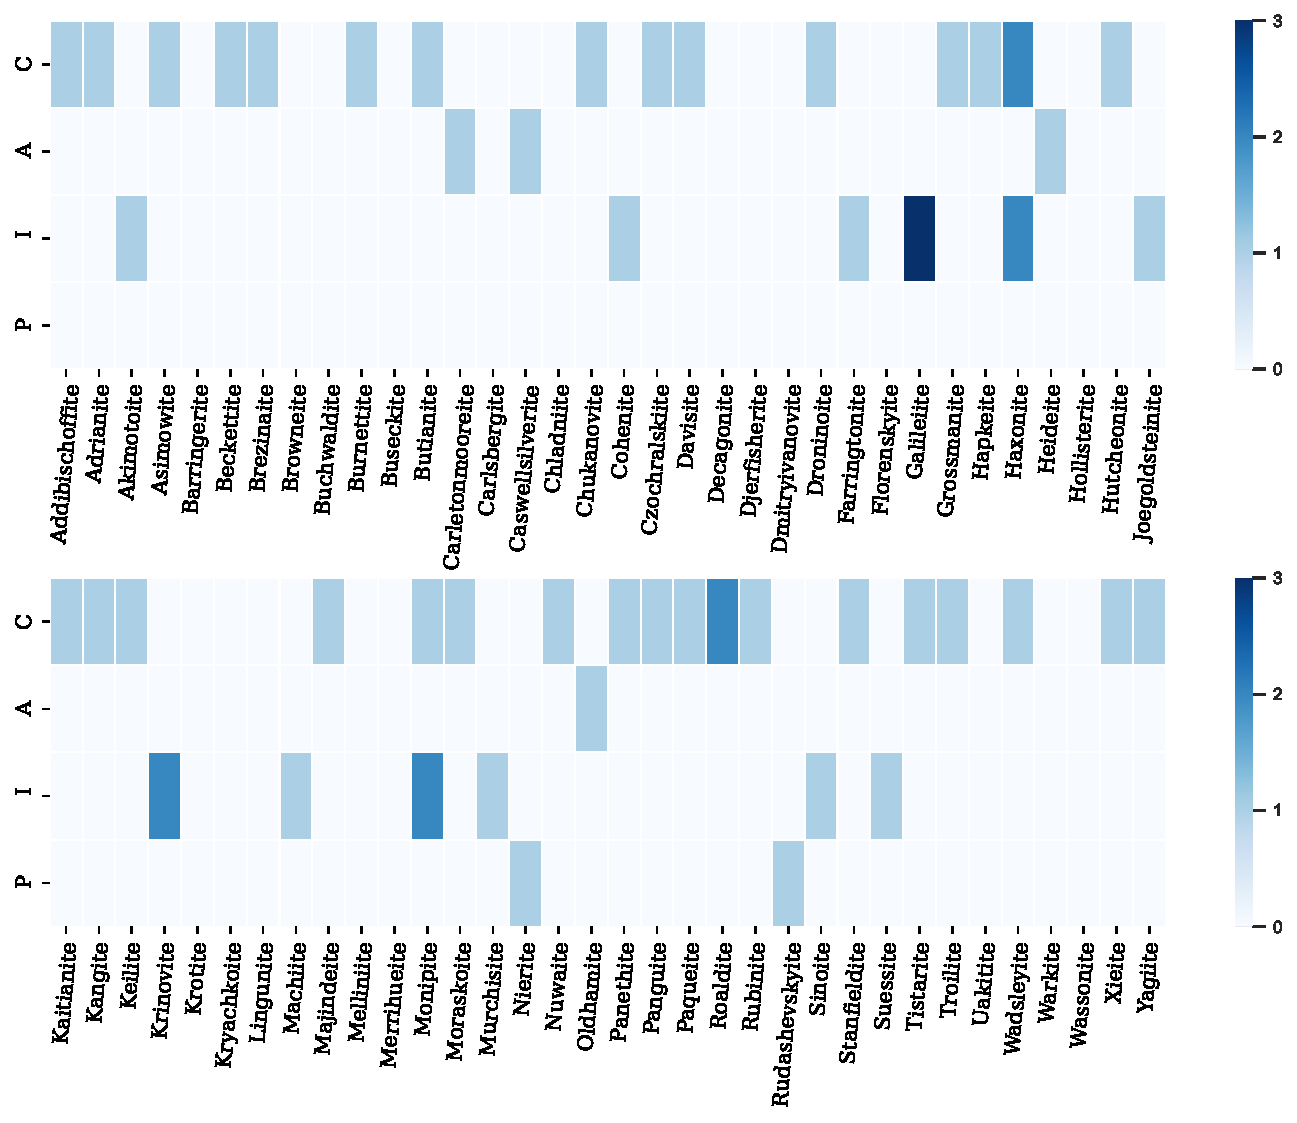
\includegraphics[width=0.75\textwidth]{mineral_dist.pdf}
    \caption{Distribution of meteorite minerals among meteorite types included in the Athena and ASU-CBM Databases, grouped by meteorite class. The ordinate labels stand for Chondrite (C), Achondrite (A), Iron (I), and Pallasite (P). These distributions are preliminary as not all known occurrences of a mineral are guaranteed to be listed in Athena.}
    \label{fig:mineralDist}
\end{figure}

%% Interesting Minerals

Some meteorite minerals have been more intensively investigated than others, and have interesting physical properties. Four examples are detailed below: 

\begin{enumerate}
    \item \textbf{Lonsdaleite} is a hexagonal polymorph of diamond and was discovered in the Canyon Diablo meteorite in 1966 \citep{FRONDEL1967}. Recent experimental evidence has confirmed that Lonsdaleite is harder than even cubic diamond \citep{VolzandGupta}. 
    \item \textbf{Panguite} discovered in the Allende meteorite and is simultaneously ``one of the oldest minerals in the Solar System” as well as an interesting candidate for high ion conductivity at elevated temperatures \citep{Ma2012}. 
    \item \textbf{Tetrataenite} has a high magnetic coercivity and has been investigated for permanent magnet applications, holding good potential as a superior rare-earth-free permanent magnet \citep{Lewis2014}.
    \item \textbf{Decagonite} is the second natural quasicrystal discovered, after icosahedrite (Al63Cu24Fe13). It is also the first to exhibit the crystallographically forbidden decagonal symmetry \citep{Bindi2015}.
\end{enumerate}

As we found it somewhat difficult to work with the relatively unstructured data repositories of varied composition, overall, we hope for a future extensive investigation that will result in the construction of an optimized database to host such information. Although the Athena mineral database was very helpful, we believe this field will benefit from a more extensive and rigorously vetted database as well as the standardization and interoperability-enhancement of current repositories.  \\

\textit{Software:} NumPy \citep{harris2020}, Matplotlib \citep{hunter2007}, and Pandas \citep{McKinney2009}. 

%\bibliographystyle{abbrv} % delete this
\bibliography{refs.bib}

\end{document}